\documentclass[11pt]{article}
\usepackage{geometry}
\geometry{margin=1in}
\usepackage{amssymb}
\usepackage{enumitem}
\usepackage{parskip}
\usepackage{xcolor}
\usepackage{tikz}
\definecolor{benblue}{HTML}{1769AA}

\newcommand{\drawbox}[1]{%
  \par\vspace{4pt}\noindent
  \fbox{\rule{0pt}{#1}\rule{\dimexpr\linewidth-2\fboxsep-2\fboxrule}{0pt}}%
  \par\vspace{6pt}}

\newcommand{\task}[1]{\par\medskip\noindent\textbf{\color{benblue}#1}\par\nopagebreak}

\title{\vspace{-1.5cm}\textbf{Circle Secrets}\\[-2pt]
  \large The inscribed angle}
\author{}
\date{}

\begin{document}
\maketitle
\vspace{-1.2cm}

\noindent\textbf{The big secret.} Pick any two points $A$ and $B$ on a circle.
The angle you see them at from a rim point $P$ is always exactly \emph{half} the
angle you see them at from the center $O$, and every rim point on the same arc
sees them at the \emph{same} angle. Today you measure it, then prove it.

\section*{Build 1: the right angle on a diameter}
Here is a circle with a diameter $AB$ and one rim point $P$.

\begin{center}
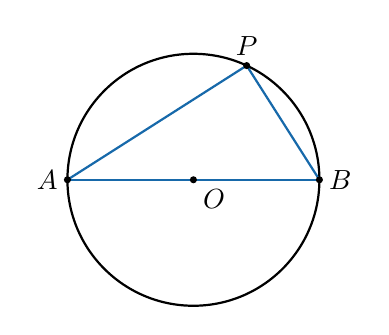
\begin{tikzpicture}[scale=0.8]
  \coordinate (O) at (0,0);
  \coordinate (A) at (-2,0);
  \coordinate (B) at (2,0);
  \coordinate (P) at (65:2);
  \draw[thick] (O) circle (2);
  \draw[benblue, thick] (A) -- (B);
  \draw[benblue, thick] (A) -- (P) -- (B);
  \fill (O) circle (1.6pt); \node[below right] at (O) {$O$};
  \fill (A) circle (1.6pt); \node[left]  at (A) {$A$};
  \fill (B) circle (1.6pt); \node[right] at (B) {$B$};
  \fill (P) circle (1.6pt); \node[above] at (P) {$P$};
\end{tikzpicture}
\end{center}

\task{Measure angle $APB$ above with a protractor: \underline{\hspace{2cm}} degrees.}
\task{Draw your own circle below with a diameter $AB$. Mark four different points
$P$ on the rim and measure angle $APB$ at each one. Do they all agree?}
\drawbox{3cm}

\section*{Build 2: the rim is half the center}
Draw a fresh circle, center $O$. Mark two points $A$ and $B$ that are \emph{not}
a diameter. Draw the center angle $AOB$. Then pick a point $P$ on the longer arc
and draw the rim angle $APB$.

\task{Center angle $AOB =$ \underline{\hspace{1.6cm}}, \quad rim angle
$APB =$ \underline{\hspace{1.6cm}}. \quad Is the rim exactly half the center?}
\drawbox{3cm}

\section*{Why is the rim half the center?}
Set it up so the line $PO$ runs straight through the center to the far side $B$
(so $PB$ is a diameter). Draw the radius $OA$ to make triangle $OAP$.

\task{$OA = OP$. Why must these two sides be equal?
\underline{\hspace{6.5cm}}}
\task{So the two base angles are equal; call each one $t$. The center angle $AOB$
is the exterior angle of the triangle at $O$, so $AOB = $
\underline{\hspace{1.8cm}} and the rim angle $APB = $ \underline{\hspace{1.8cm}}.
The rim is half the center.}
\drawbox{1.5cm}

\section*{Push further}
\begin{enumerate}[leftmargin=*]
  \item \textbf{Thales for free.} If $AB$ is a diameter, the center angle is the
        straight line $180^\circ$, so the rim angle must be
        \underline{\hspace{1.6cm}} degrees.
  \item \textbf{Cyclic quadrilateral (BMC gold).} Put four points on a circle and
        join them into a quadrilateral. Opposite angles add to
        \underline{\hspace{1.6cm}}. Prove it: each corner stands on an arc, and
        the four arcs cover the whole circle ($360^\circ$).
  \item \textbf{Competition gem.} Two chords $AB$ and $CD$ cross at a point $X$
        inside the circle. Show that triangle $AXC$ and triangle $DXB$ have the
        same shape (similar). Hint: find two pairs of equal inscribed angles on
        the same arcs. This gives the length rule $AX \cdot XB = CX \cdot XD$.
\end{enumerate}

\task{Draw the cyclic quadrilateral and the crossing chords here:}
\drawbox{3.2cm}

\end{document}
